\documentclass[tikz,margin=1mm]{standalone}
% show the minority charge carriers in the regions coming from the regions where they are the majority
% rand produces a number uniformly randomly between -1 and 1
% 5 x zoom of the previous figure

\def\crt{1.255921} % cube root of two
\def\fact{.4}
% with appropriate scaling and dimensions, the \fact could be made unity and removed

\usetikzlibrary{calc}

\begin{document}
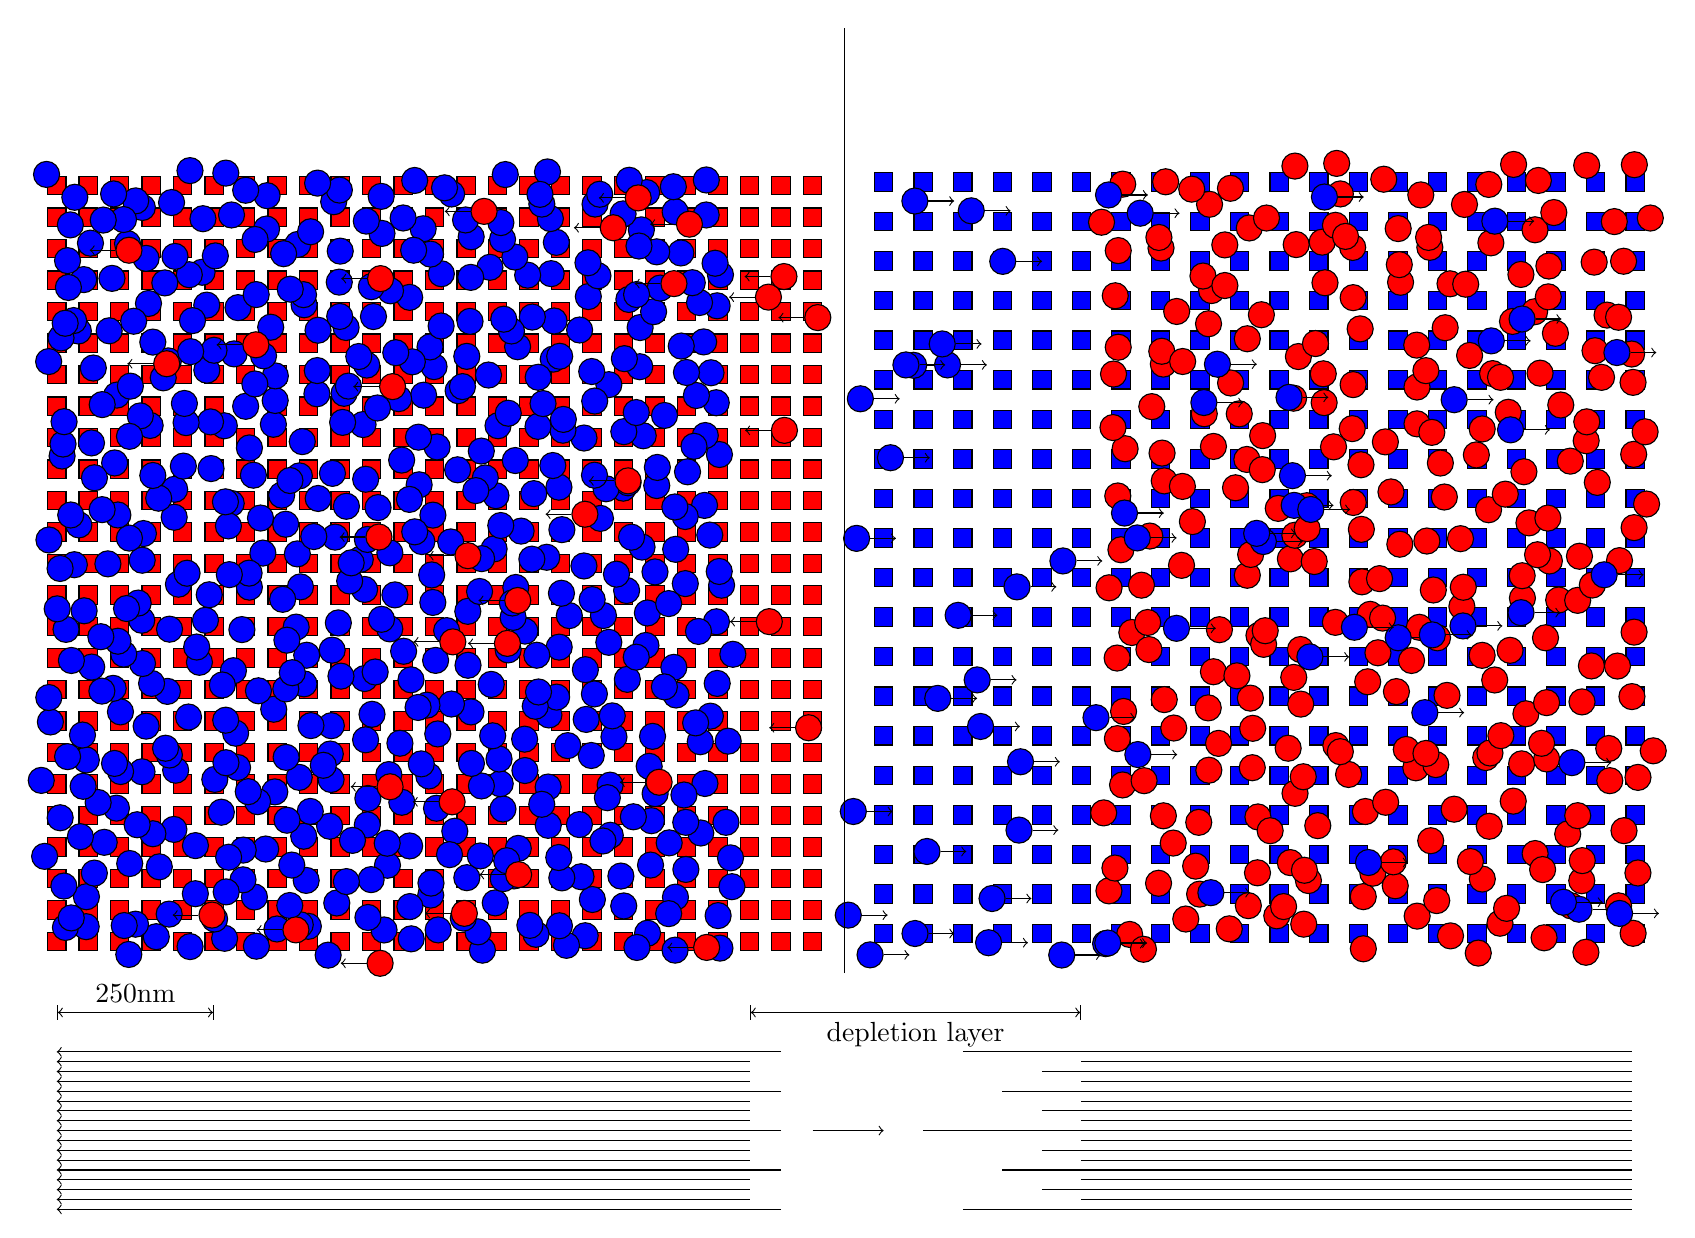
\begin{tikzpicture}
%% dopant "lattices" (simplification)
\foreach\x in {-1,-2,-3,...,-25}
  \foreach\y in {1,2,3,...,25}
    {
    \node[draw, minimum size=.1cm, fill=red] at ($(\fact*\x,\fact*\y)$) {};
    }

\foreach\x in {-4,-5,-6,-7,-8,...,-25} % 1--3 is depletion (field effect reduces depletion width)
  \foreach\y in {1,2,3,...,25} 
    {
    \node[circle, draw, minimum size=.05cm, fill=blue] at ($(\fact*\x,\fact*\y) + (\fact*rand/2,\fact*rand/2)$) {};
    }
%
% majority free carriers on either side
\begin{scope}
\foreach\x in {1,2,3,...,20}
  \foreach\y in {1,2,3,...,20}
    {
    \node[draw, minimum size=.1cm, fill=blue] at ($(\fact*\crt*\x,\fact*\crt*\y)$) {};
    }
\foreach\x in {7,8,9,10,11,12,13,...,20} % 1--6 is depletion based on 2x volume, note though, that this will give 2*2**(1/3) the distance
  \foreach\y in {1,2,3,...,20}
    {
    \node[circle, draw, minimum size=.05cm, fill=red] at ($(\fact*\crt*\x,\fact*\crt*\y) + (\fact*\crt*rand/2,\fact*\crt*rand/2)$) {};
    }
\end{scope}
%
% minority carriers on opposite sides
% how many more minority carriers are there? there is actually a diffusion current density whose dependence is a function of distance
% but within the depletion region, which limits the current, they are proportional to the dopant densities
% assume twice as dense (
\foreach\x in {1,2,3,...,32}
    {
    \node[circle, draw, minimum size=.05cm, fill=red] (a) at ($(-5,5) + (-5*rand,5*rand)$) {};
    \draw[->] (a) --++ (-.5,0);
    }

\foreach\x in {1,2,3,...,64}
    {
    \node[circle, draw, minimum size=.05cm, fill=blue] (a) at ($(5,5) + (5*rand,5*rand)$) {};
    \draw[->] (a) --++ (.5,0);
    }

% auxillary and electric field

% nominal junction
\draw (0, 0) -- (0, 12);

% scale bar
\draw[|<->|] (-10, -0.5) -- (-8,-0.5) node[pos=0.5, above] {250nm};

% depletion layer label
\draw[|<->|,align=center] (\fact*-3,-.5) -- (\fact*\crt*6,-.5) node[pos=0.5, below] {depletion layer};

% electric field
\def\os{-3}
\draw[->] (-\fact, \os + 8/8) -- (\fact*\crt, \os + 8/8);
% opposing field from (-\fact, \fact*\crt)

% left side
% from x = (-2*\fact,-\fact) the net electric field is zero
% first

\draw[->] (-2*\fact, \os + 0/8) -- (-25*\fact, \os + 0/8);
\draw[->] (-2*\fact, \os + 4/8) -- (-25*\fact, \os + 4/8);
\draw[->] (-2*\fact, \os + 8/8) -- (-25*\fact, \os + 8/8);
\draw[->] (-2*\fact, \os + 12/8) -- (-25*\fact, \os + 12/8);
\draw[->] (-2*\fact, \os + 16/8) -- (-25*\fact, \os + 16/8);
% second
\draw[->] (-3*\fact, \os + 2/8) -- (-25*\fact, \os + 2/8);
\draw[->] (-3*\fact, \os + 6/8) -- (-25*\fact, \os + 6/8);
\draw[->] (-3*\fact, \os + 10/8) -- (-25*\fact, \os + 10/8);
\draw[->] (-3*\fact, \os + 14/8) -- (-25*\fact, \os + 14/8);
%
\draw[->] (-3*\fact, \os + 1/8) -- (-25*\fact, \os + 1/8);
\draw[->] (-3*\fact, \os + 3/8) -- (-25*\fact, \os + 3/8);
\draw[->] (-3*\fact, \os + 5/8) -- (-25*\fact, \os + 5/8);
\draw[->] (-3*\fact, \os + 7/8) -- (-25*\fact, \os + 7/8);
\draw[->] (-3*\fact, \os + 9/8) -- (-25*\fact, \os + 9/8);
\draw[->] (-3*\fact, \os + 11/8) -- (-25*\fact, \os + 11/8);
\draw[->] (-3*\fact, \os + 13/8) -- (-25*\fact, \os + 13/8);
\draw[->] (-3*\fact, \os + 15/8) -- (-25*\fact, \os + 15/8);

% from x=(\fact*\crt, 2*\fact*\crt) the net electric field is zero
\draw[] (2*\fact*\crt, \os + 8/8) -- (25*\fact, \os + 8/8);
%
\draw[] (3*\fact*\crt, \os + 0/8) -- (25*\fact, \os + 0/8);
\draw[] (3*\fact*\crt, \os + 16/8) -- (25*\fact, \os + 16/8);
%
\draw[] (4*\fact*\crt, \os + 4/8) -- (25*\fact, \os + 4/8);
\draw[] (4*\fact*\crt, \os + 12/8) -- (25*\fact, \os + 12/8);
%%
\draw[] (5*\fact*\crt, \os + 2/8) -- (25*\fact, \os + 2/8);
\draw[] (5*\fact*\crt, \os + 6/8) -- (25*\fact, \os + 6/8);
\draw[] (5*\fact*\crt, \os + 10/8) -- (25*\fact, \os + 10/8);
\draw[] (5*\fact*\crt, \os + 14/8) -- (25*\fact, \os + 14/8);
%%
\draw[] (6*\fact*\crt, \os + 1/8) -- (25*\fact, \os + 1/8);
\draw[] (6*\fact*\crt, \os + 3/8) -- (25*\fact, \os + 3/8);
\draw[] (6*\fact*\crt, \os + 5/8) -- (25*\fact, \os + 5/8);
\draw[] (6*\fact*\crt, \os + 7/8) -- (25*\fact, \os + 7/8);
\draw[] (6*\fact*\crt, \os + 9/8) -- (25*\fact, \os + 9/8);
\draw[] (6*\fact*\crt, \os + 11/8) -- (25*\fact, \os + 11/8);
\draw[] (6*\fact*\crt, \os + 13/8) -- (25*\fact, \os + 13/8);
\draw[] (6*\fact*\crt, \os + 15/8) -- (25*\fact, \os + 15/8);

\end{tikzpicture}

\end{document}
